\documentclass[12pt,a4paper]{article}

% -------------------- Page Layout --------------------
\usepackage[
top=2.5cm,
bottom=2.5cm,
left=2.5cm,
right=2.5cm
]{geometry}

% -------------------- Math Packages --------------------
\usepackage{amsmath,amssymb}

% -------------------- Figures --------------------
\usepackage{graphicx}
\usepackage{float}
\usepackage{caption}

% -------------------- Formatting --------------------
\usepackage{setspace}
\usepackage{enumitem}
\usepackage{titlesec}
\usepackage{xcolor}
\usepackage{hyperref}

% -------------------- Fonts --------------------
\usepackage{fontspec}
\setmainfont{Times New Roman}

% -------------------- General Settings --------------------
\onehalfspacing
\setlength{\parindent}{0pt}
\setlength{\parskip}{0.75em}

\graphicspath{{outputs/figures/}}

\hypersetup{
	colorlinks=true,
	linkcolor=blue,
	urlcolor=blue,
	citecolor=blue
}

\captionsetup{
	font=small,
	labelfont=bf,
	justification=centering
}

\titleformat{\section}
{\Large\bfseries}
{}
{0pt}
{}

\titleformat{\subsection}
{\large\bfseries}
{}
{0pt}
{}

\titleformat{\subsubsection}
{\normalsize\bfseries}
{}
{0pt}
{}

\setlist[itemize]{
	topsep=0.4em,
	itemsep=0.45em,
	parsep=0pt,
	leftmargin=1.5em
}

% -------------------- Document --------------------
\begin{document}
	
	\begin{titlepage}
		\centering
		
		\vspace*{1cm}
		
		{\Huge\bfseries Third Project of Mathematical Software Course\par}
		\vspace{1.2cm}
		
		{\Large Numerical Methods\par}
		\vspace{2.3cm}
		
		\rule{0.75\textwidth}{0.8pt}\par
		\vspace{1cm}
		
		{\Large\bfseries Ali Taghizadeh\par}
		
		\vspace{1.2cm}
		
		{\large\bfseries Student ID:\par}
		\vspace{0.45cm}
		{\large 40313008\par}
		
		\vspace{0.8cm}
		
		\vspace{0.8cm}
		
		\vspace{0.8cm}
		
		{\large\bfseries GitHub Repository Link:\par}
		\vspace{0.35cm}
		{\large\href{https://github.com/alitkbbl/Numerical-Methods}{github.com/alitkbbl/Numerical-Methods}\par}
		
		\vfill
		
		\rule{0.75\textwidth}{0.8pt}\par
		\vspace{0.8cm}
		
		{\large \today\par}
		
	\end{titlepage}
	
	\newpage
	
	% ==================== Question 1 ====================
	\section*{Question 1: Lagrange Interpolation and Spline}
	
	In this section, the goal is to find a function for the following set of points that passes through all of them:
	\[
	(1,1),\ (2,3),\ (3,5),\ (4,8),\ (5,5),\ (6,2)
	\]
	For this purpose, two methods were used: Lagrange interpolation and cubic spline interpolation
	(Cubic Spline).
	The program output shows that both methods have been implemented correctly, because the error at the given nodes is zero and both functions pass exactly through the original points.
	
	\subsection*{Implementation Details}
	
	To interpolate these six points, two main methods were examined:
	
	\textbf{1. Lagrange Polynomial:}
	In this method, the function
	\texttt{scipy.interpolate.lagrange}
	was used. This function constructs a unique polynomial that passes through all the given points. Since in the Lagrange method only one polynomial is constructed over the entire interval, the final output is a global and smooth function; however, this same property can sometimes cause unwanted oscillations, especially near the endpoints of the interval.
	
	\textbf{2. Natural Cubic Spline:}
	For this part, the
	\texttt{CubicSpline}
	class was used. In spline interpolation, instead of constructing a single polynomial for all points, a separate cubic polynomial is defined between each pair of consecutive points. Therefore, the final function is constructed piecewise and usually has a more natural and controlled behavior between the points.
	
	\textbf{Validation of Results:}
	To ensure the correctness of the implementation, the values of both functions at the original data points were checked. The result showed that both methods pass exactly through the given points. Also, using
	\texttt{sympy},
	the symbolic forms of the functions were extracted so that, in addition to the plots, their analytical representations would also be available.
	
	\textbf{Visualization and Comparison:}
	Finally, the curves of both methods were plotted together with the original points. This comparison helps to better observe the behavioral differences between the two methods: Lagrange constructs a unique global polynomial, while the spline, with its piecewise structure, usually has fewer oscillations and is a more reliable choice for many real-world datasets.
		\newpage
	\subsection*{1. Formulas of the Obtained Functions}
	
	\textbf{a) Lagrange Interpolation}
	
	Since 6 points are given, the Lagrange polynomial will be of degree 5. After calculation and simplification, the polynomial formula was obtained as follows:
	
	\begin{equation}
		P(x)=
		0.175x^5
		- 2.958x^4
		+ 18.375x^3
		- 52.041x^2
		+ 68.45x
		- 31.0
	\end{equation}
	
	\textbf{b) Cubic Spline Interpolation}
	
	In the cubic spline method, the final function consists of third-degree polynomials. These polynomials are connected at the nodes, and in addition to the function values, their first and second derivatives are also continuous at the connection points. As an example, the formula of the function on the first interval, namely
	$[1,2]$,
	was calculated as follows:
	
	\begin{equation}
		S_0(x)=
		-0.186x^3
		+ 0.559x^2
		+ 1.626x
		- 1.0
	\end{equation}
	
	The formulas for the other intervals are also fully included in the program output.
	
	\subsection*{2. Plot Analysis and Comparison of the Two Methods}
	
	According to the plot in Figure
	\ref{fig:q1_interpolation},
	the difference in the behavior of the two methods is clearly visible:
	
	\begin{itemize}
		\item \textbf{Lagrange behavior:}
		The Lagrange curve, shown in blue, is a fifth-degree polynomial. This curve passes through all the points, but because the polynomial is global, it shows more oscillation in some parts. This issue is especially more visible in the final interval between
		$x=5$
		and
		$x=6$.
		Such behavior is an example of Runge's Phenomenon in polynomial interpolation.
		
		\item \textbf{Spline behavior:}
		In contrast, the cubic spline, shown with a red dashed line, follows a smoother and more natural path between the points. Since this method works piecewise and uses only one third-degree polynomial in each interval, it creates fewer artificial oscillations. Therefore, for such data, the spline is usually a more suitable choice.
	\end{itemize}
	
	\begin{figure}[H]
		\centering
		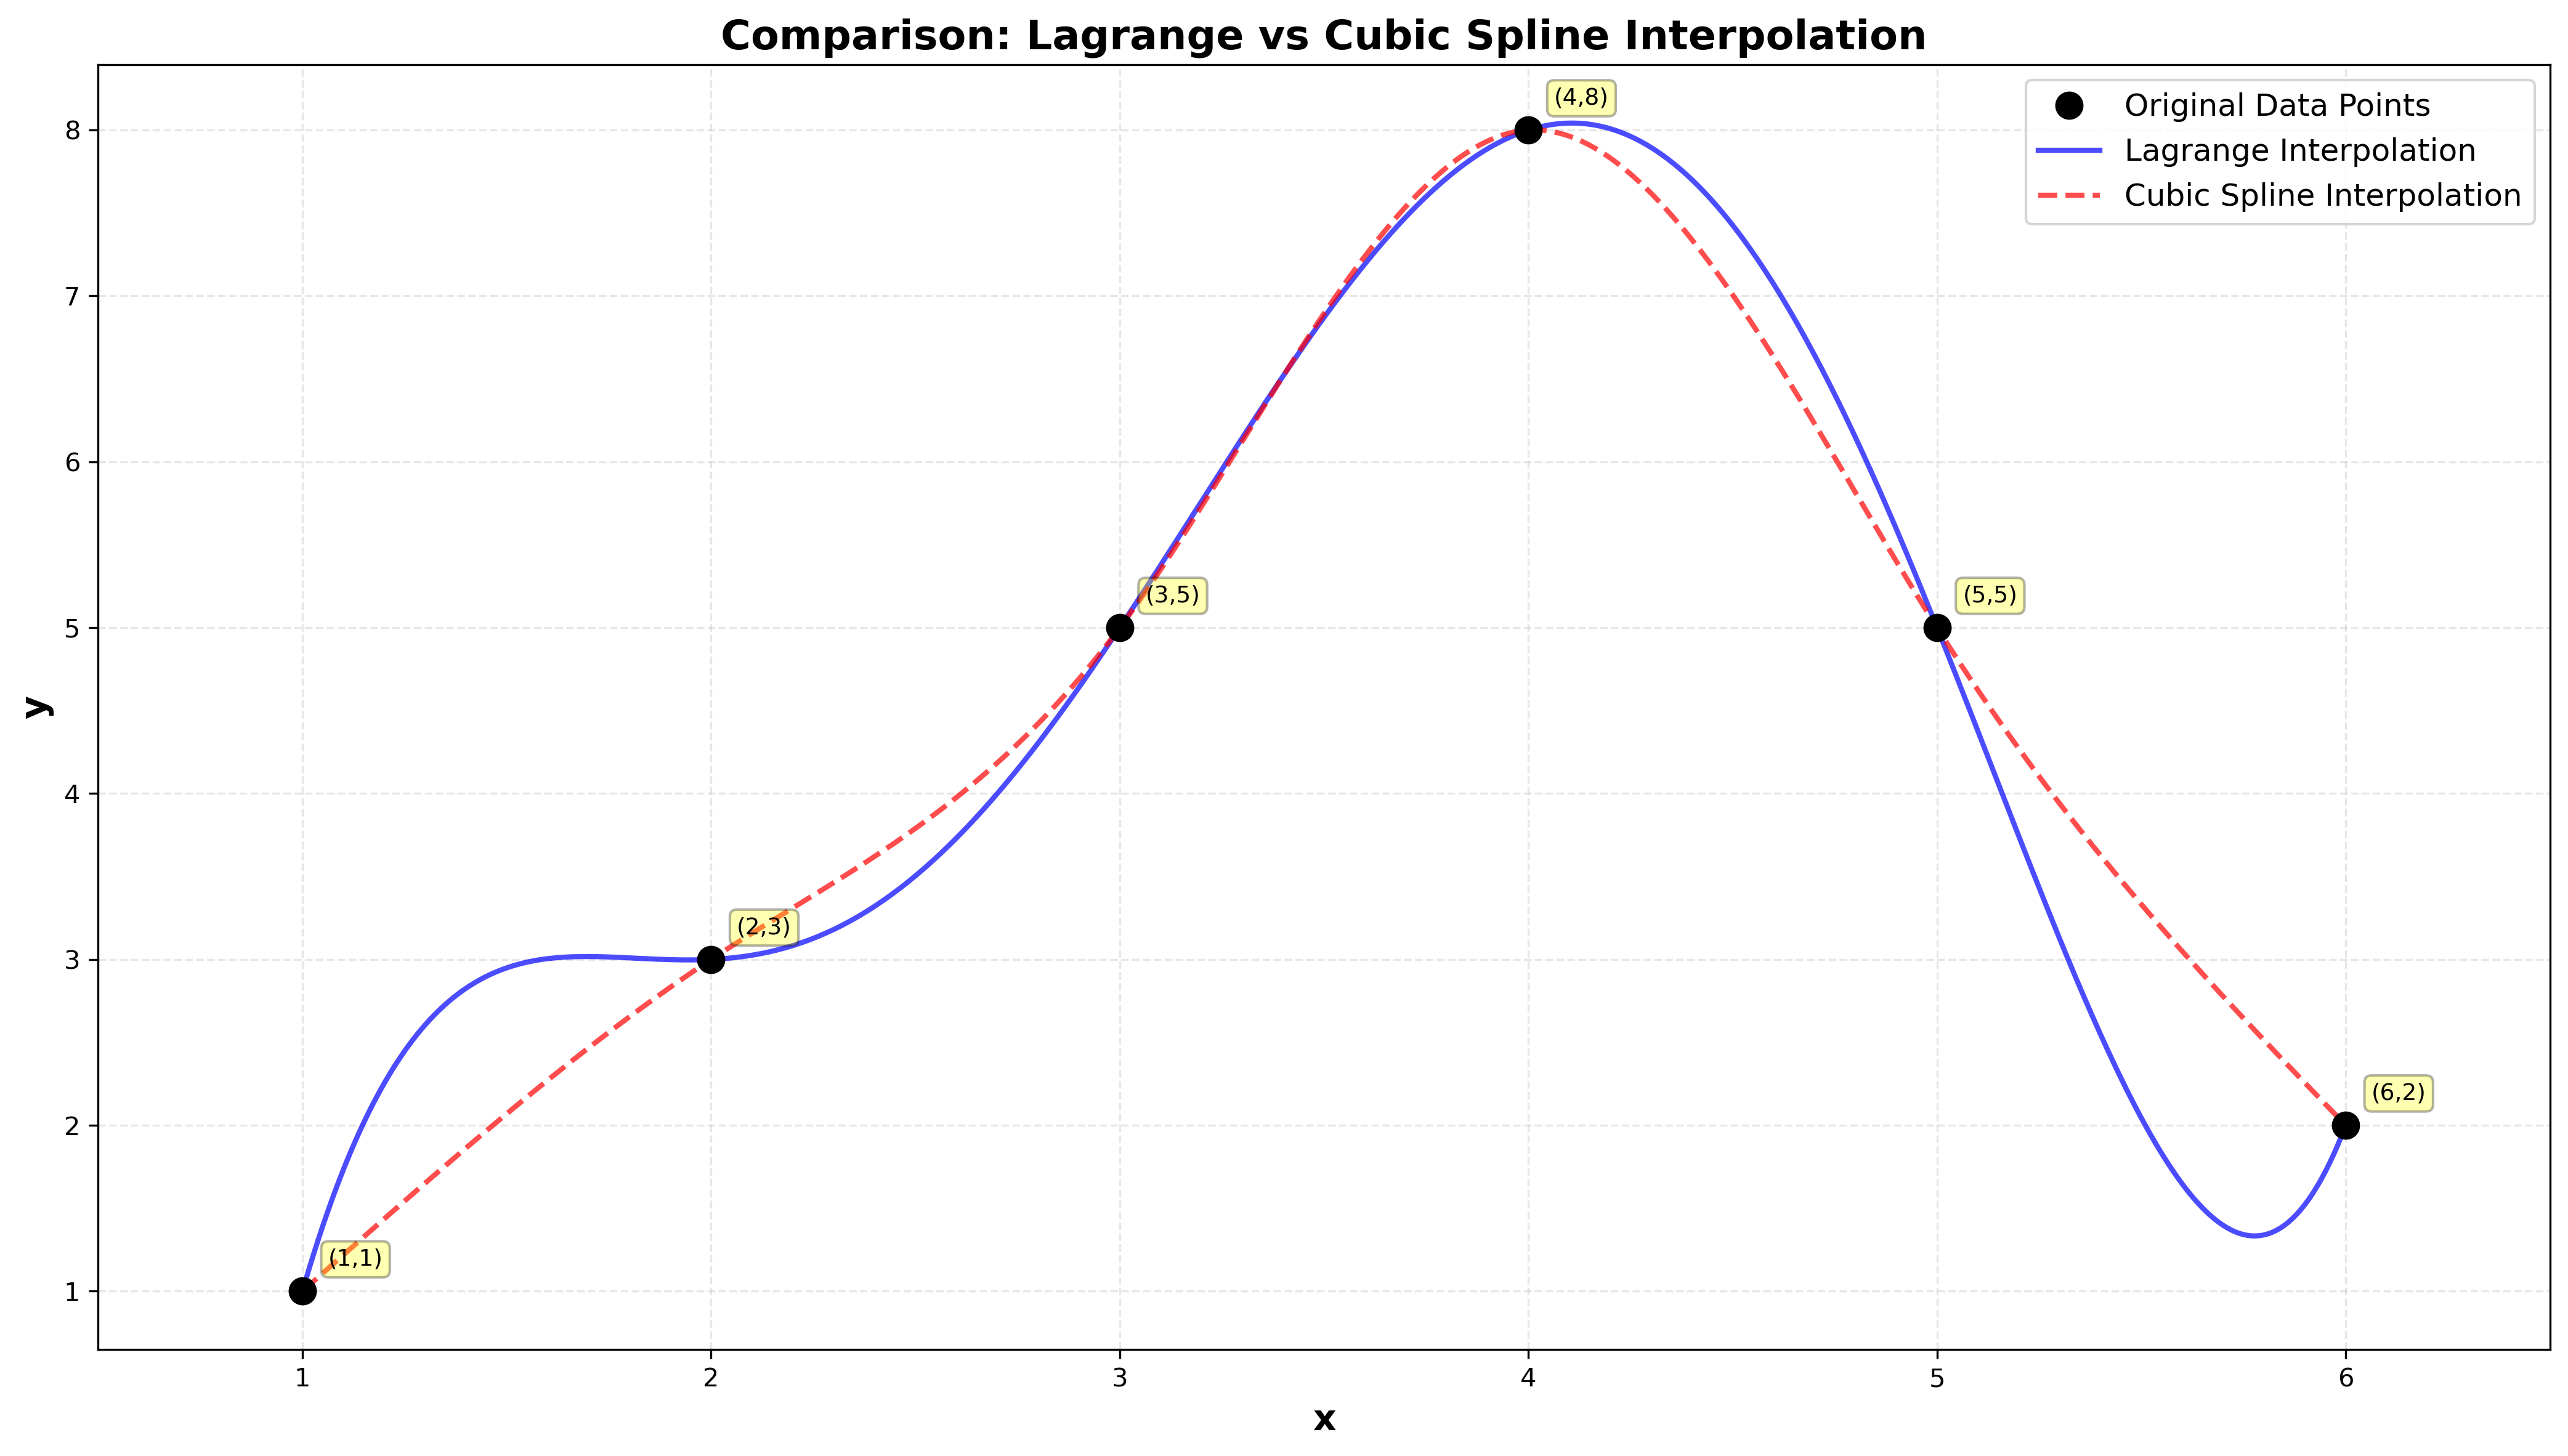
\includegraphics[width=0.88\textwidth]{../outputs/figures/question1_interpolation.png}
		\caption{Comparison of Lagrange interpolation and cubic spline on the given data points}
		\label{fig:q1_interpolation}
	\end{figure}
	
	
	\newpage
	% ==================== Question 2 ====================
	\section*{Question 2: Visualization and Runtime Analysis of Algorithms}
	
	In this section, the execution time of three algorithms
	(Alg.1, Alg.2, Alg.3)
	was examined for datasets with sizes from
	$100\,\text{KB}$
	to
	$700\,\text{KB}$.
	The data were read from an Excel file, and the code structure was written in such a way that when new data are added, such as the row corresponding to
	$700\,\text{KB}$,
	the calculations and plots are updated without requiring major changes to the program.
	
	\subsection*{Implementation Details}
	
	In this question, the data related to the execution times of the algorithms were read directly from the Excel file. For this purpose, the
	\texttt{pandas.read\_excel}
	function was used so that the information would be imported into the program in an organized form. Reading rows and columns was also done dynamically so that the code would be flexible against the addition of new data.
	
	\textbf{Data Visualization:}
	To make the behavior of the algorithms easier to compare, three types of plots were generated:
	
	\begin{itemize}
		\item \textbf{Bar chart:} for direct comparison of algorithm execution times at different data sizes
		\item \textbf{Line chart:} for observing the growth trend of execution time and examining the overall behavior of each algorithm
		\item \textbf{Box plot:} for examining dispersion, stability, and statistical differences in the execution times of the algorithms
	\end{itemize}
	
	\textbf{Statistical Calculations:}
	For each algorithm, the main statistical indicators, including mean, median, and standard deviation, were calculated. Also, the average execution time of Algorithm 2 in the range
	$100\,\text{KB}$
	to
	$600\,\text{KB}$
	was calculated separately. This calculation was performed by filtering the
	\texttt{DataFrame}
	based on data size.
	
	Overall, the code was designed so that both in the data processing section and in the plotting section, it has little dependence on the number of records and can work well with new inputs.
	
	\subsection*{a and b) Plotting the Charts and Analyzing the Behavior of the Algorithms}
	
	Based on the 7 records available in the data, the behavior of the three algorithms can be analyzed as follows:
	
	\begin{itemize}
		\item \textbf{Algorithm Alg.1:}
		This algorithm has the best performance among the three algorithms. Its execution time for the
		$100\,\text{KB}$
		data is
		$50\,\text{ms}$,
		and even for the largest input, namely
		$700\,\text{KB}$,
		it only reaches
		$80\,\text{ms}$.
		The growth of execution time in this algorithm is very slow, and for each
		$100\,\text{KB}$,
		it increases by approximately
		$5\,\text{ms}$.
		Its average execution time is
		$65\,\text{ms}$,
		and its standard deviation is
		$10\,\text{ms}$,
		which indicates the very good stability of the algorithm.
		
		\item \textbf{Algorithm Alg.2:}
		This algorithm initially has a higher execution time than the other two algorithms and starts from
		$200\,\text{ms}$
		for the
		$100\,\text{KB}$
		data. However, its growth slope is relatively mild, and it increases by only
		$20\,\text{ms}$
		at each step. The average execution time of this algorithm over all data is
		$260\,\text{ms}$.
		Therefore, although it starts slower, for larger data it has more acceptable behavior compared to the third algorithm.
		
		\item \textbf{Algorithm Alg.3:}
		For the small
		$100\,\text{KB}$
		data, this algorithm has better performance than
		Alg.2
		with an execution time of
		$100\,\text{ms}$,
		but its main problem is the high growth rate of execution time. Its execution time increases by about
		$100\,\text{ms}$
		at each step and reaches
		$700\,\text{ms}$
		for the
		$700\,\text{KB}$
		data. Its average execution time is
		$400\,\text{ms}$,
		and its standard deviation is
		$200\,\text{ms}$,
		which shows that this algorithm is highly sensitive to the increase in data size.
	\end{itemize}
	
	An interesting statistical point is that since the execution time of all three algorithms follows a completely linear and regular trend, the values of the
	Mean
	and
	Median
	for each algorithm are equal.
	
	\subsubsection*{Review of the Plotted Charts}
	
	For a more detailed analysis, three main charts were plotted.
	
	\textbf{1. Line Chart}
	
	In Figure
	\ref{fig:q2_line_chart},
	the growth trend of the execution time of all three algorithms is shown. The most important point in this chart is the intersection of the
	Alg.2
	and
	Alg.3
	lines at the size of
	$200\,\text{KB}$.
	This point shows that for data smaller than 200 kilobytes, the third algorithm can be a better option; however, after that point, the second algorithm performs better due to its lower growth slope.
	
	\begin{figure}[H]
		\centering
		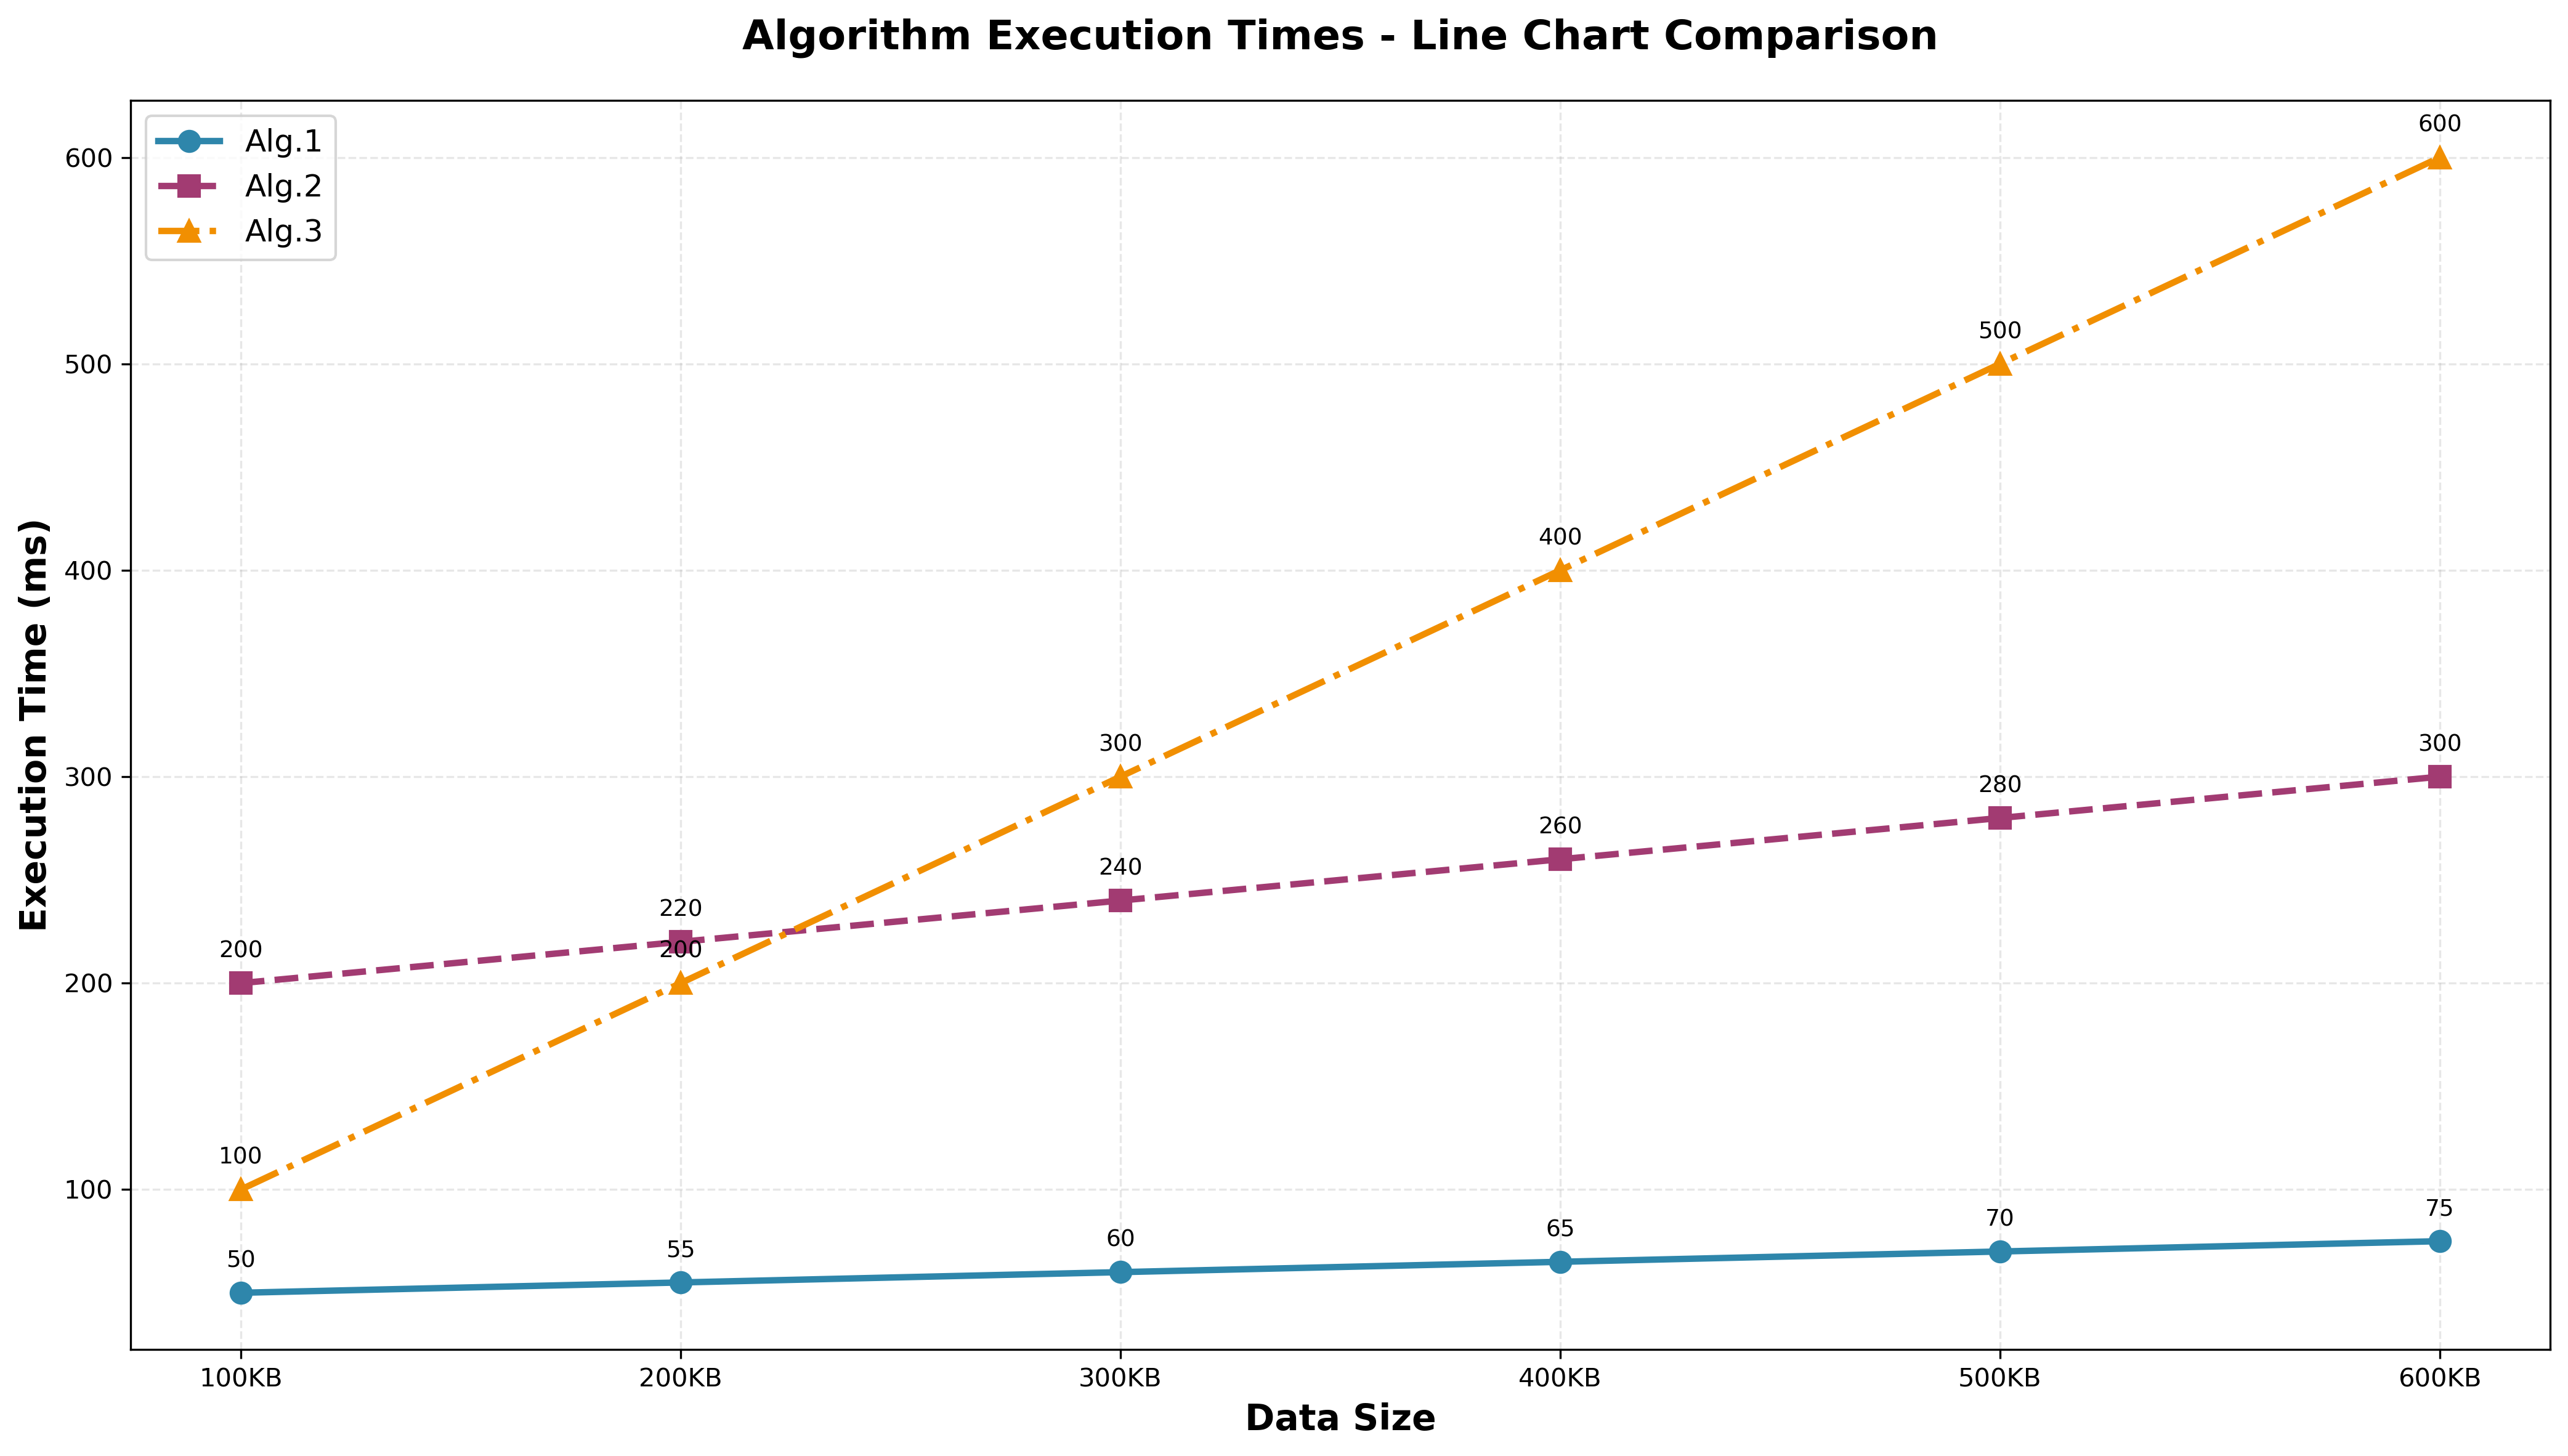
\includegraphics[width=0.88\textwidth]{../outputs/figures/question2_line_chart.png}
		\caption{Line chart comparing algorithm execution time based on data size}
		\label{fig:q2_line_chart}
	\end{figure}
	
	\textbf{2. Bar Chart}
	
	Figure
	\ref{fig:q2_bar_chart}
	shows the point-by-point comparison of the algorithms. In this chart, it is clearly visible that the bars corresponding to
	Alg.3
	grow much faster than the other two algorithms as the data size increases. At the end of the chart, the difference between this algorithm and the other two methods is completely noticeable.
	
	\begin{figure}[H]
		\centering
		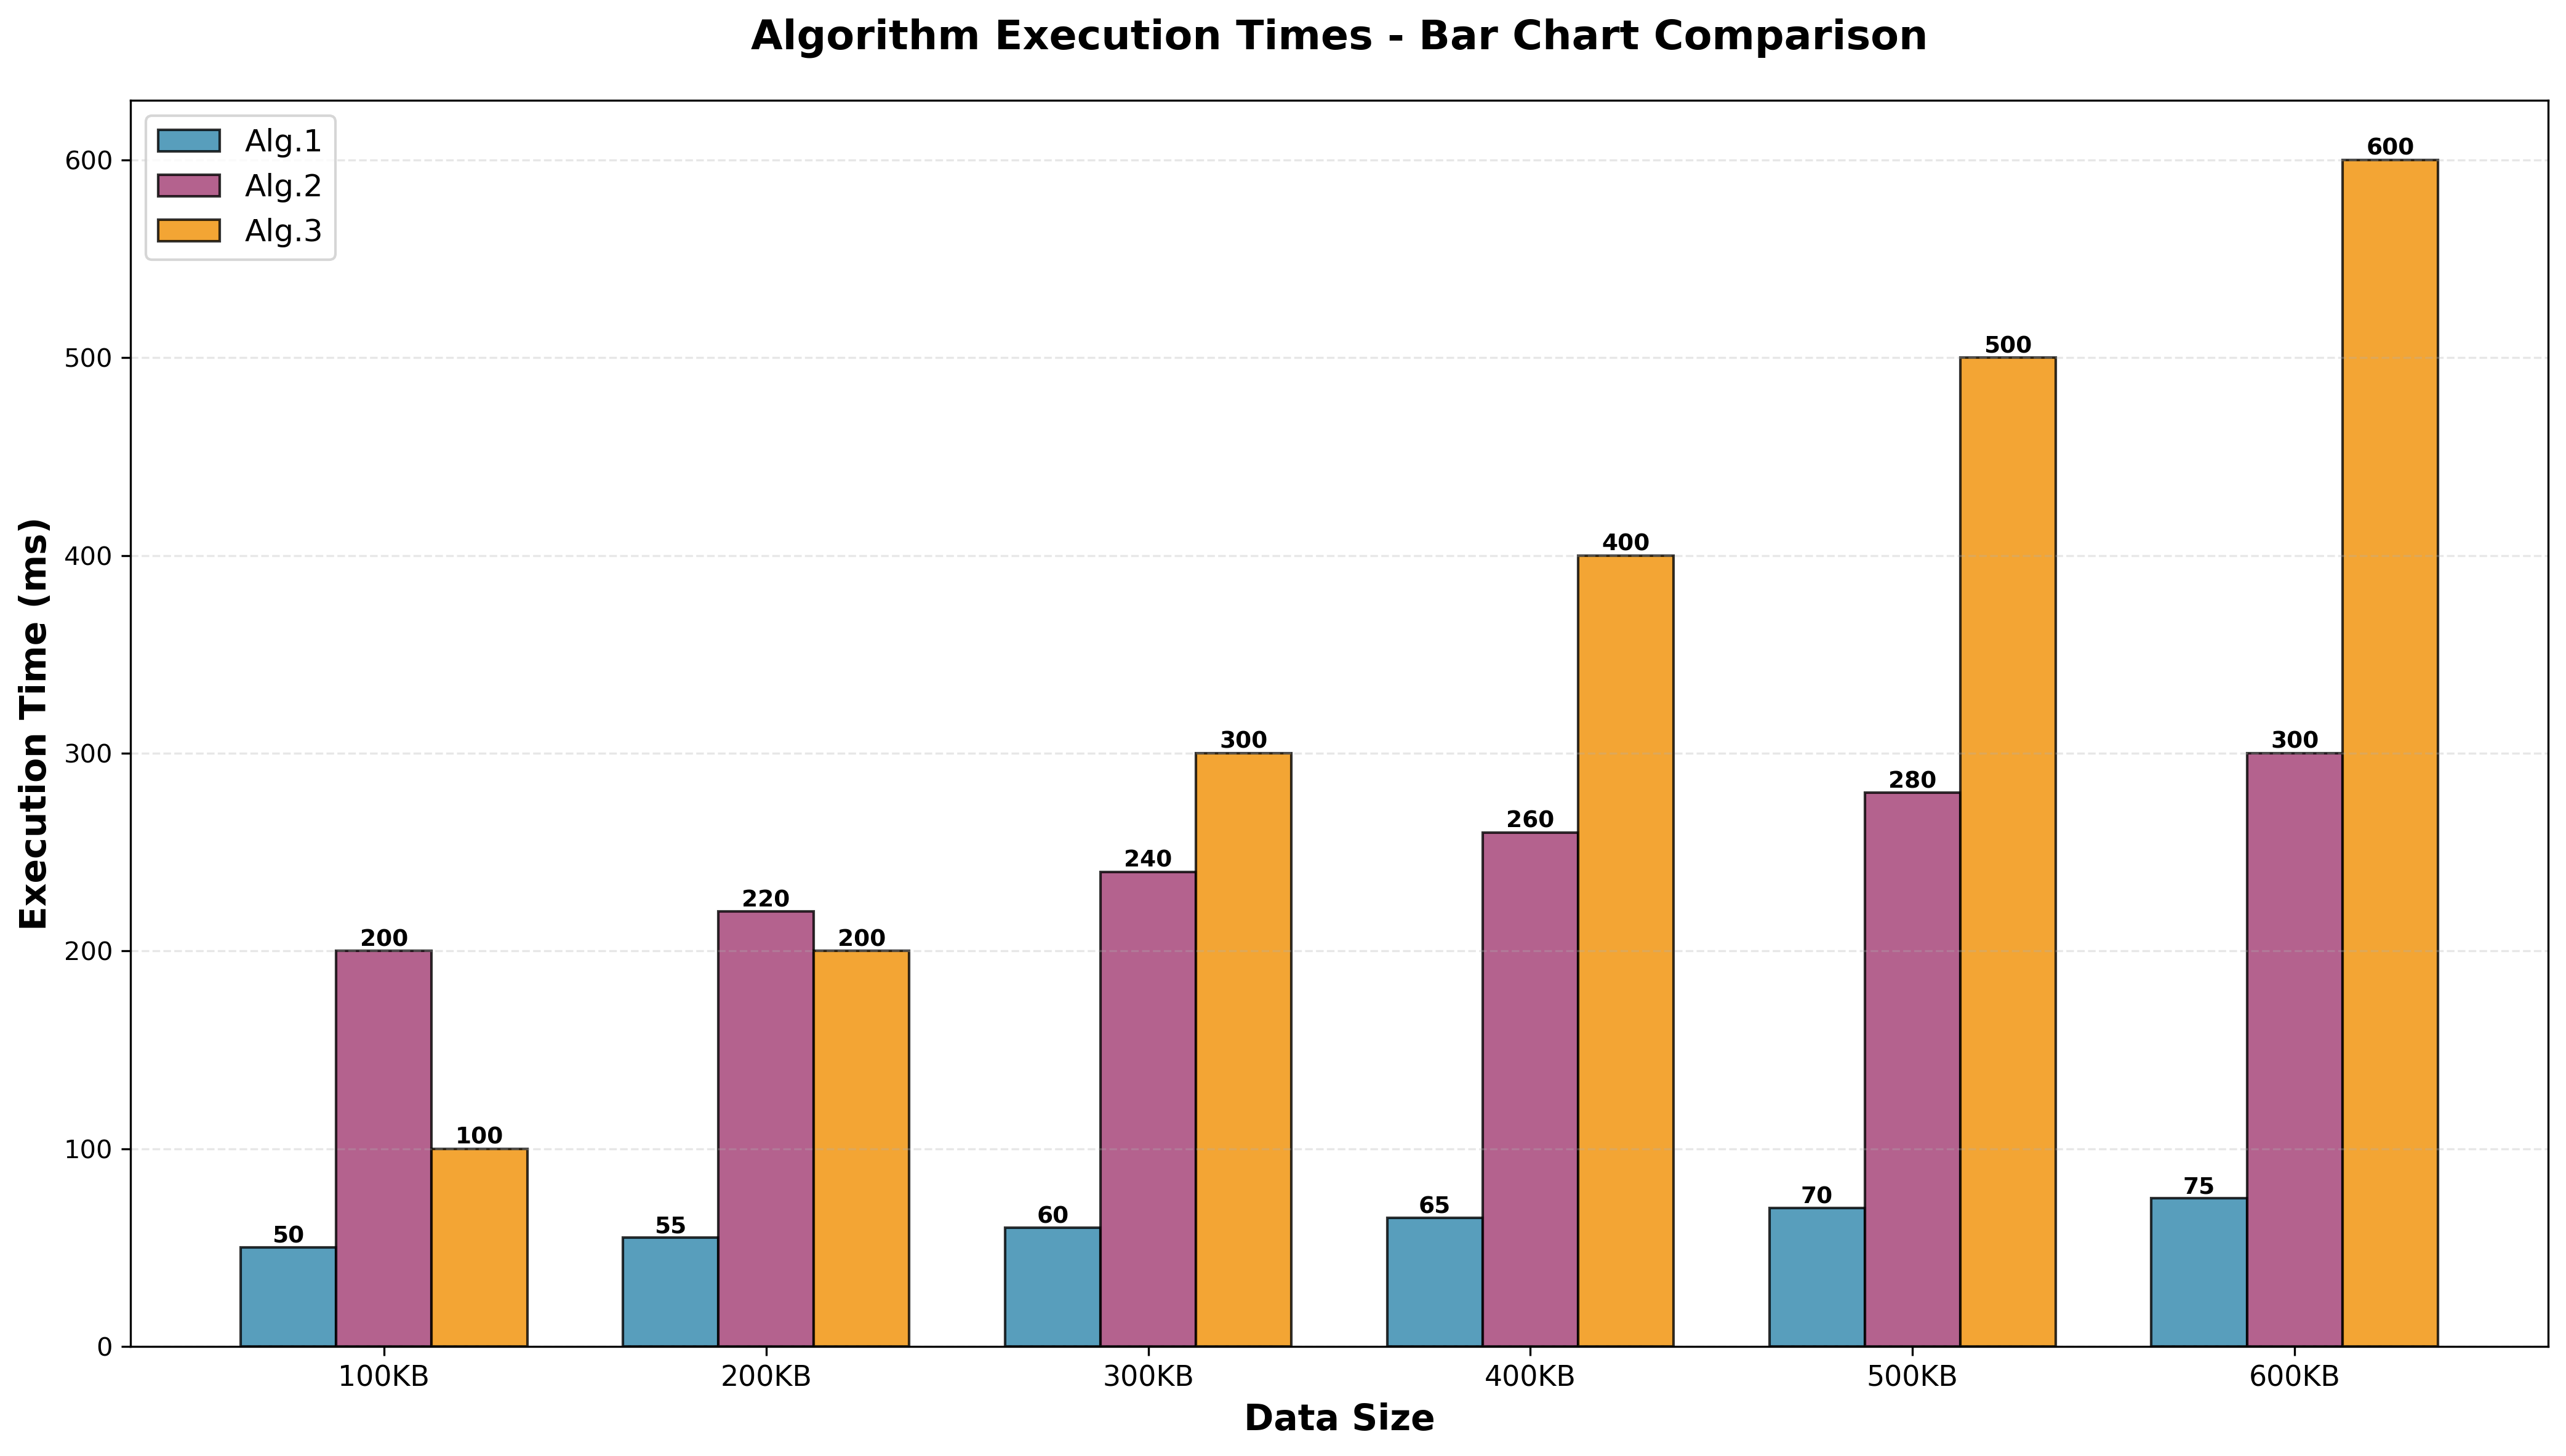
\includegraphics[width=0.88\textwidth]{../outputs/figures/question2_bar_chart.png}
		\caption{Bar chart of algorithm execution times by data size}
		\label{fig:q2_bar_chart}
	\end{figure}
	
	\textbf{3. Box Plot}
	
	Figure
	\ref{fig:q2_box_plot}
	was plotted to examine the dispersion of execution times. The small size of the box corresponding to
	Alg.1
	shows that the execution time of this algorithm does not change much for different data sizes. In contrast, the large spread of the
	Alg.3
	box indicates high dispersion and high sensitivity to the input data size. Also, the placement of the mean on the median in all three charts confirms the linear and symmetric nature of the data.
	
	\begin{figure}[H]
		\centering
		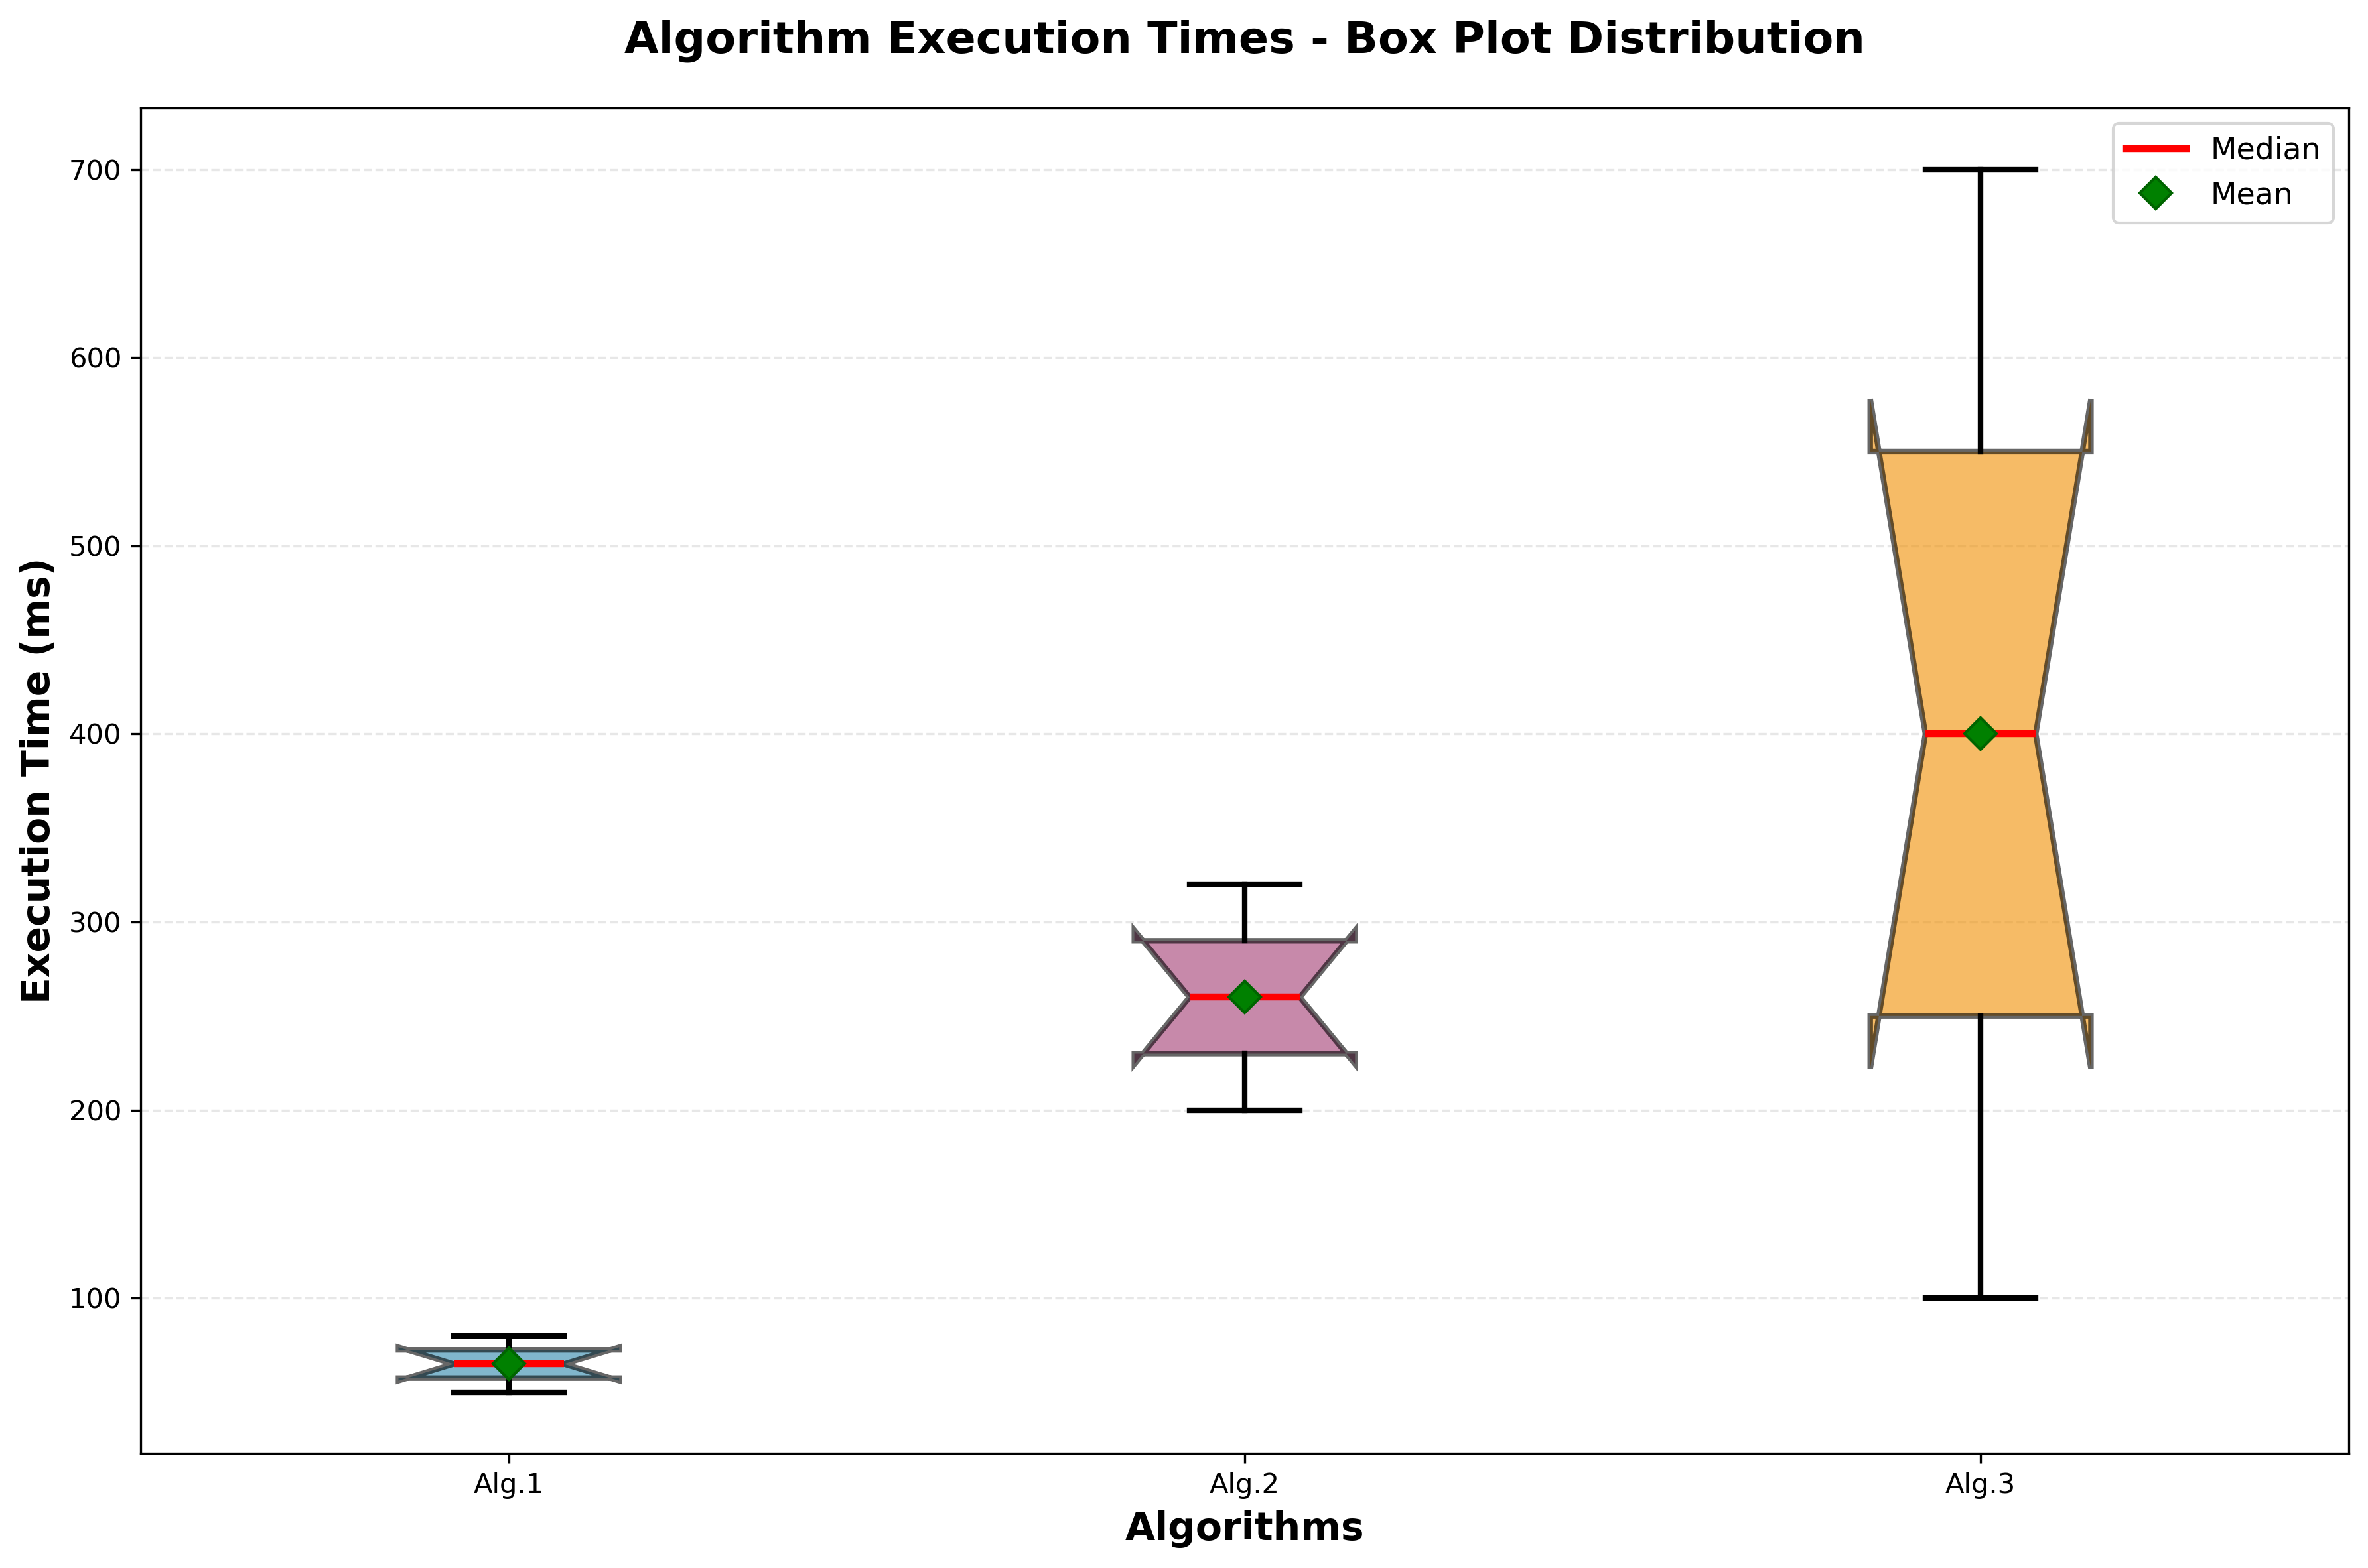
\includegraphics[width=0.88\textwidth]{../outputs/figures/question2_box_plot.png}
		\caption{Box plot of the dispersion of algorithm execution times}
		\label{fig:q2_box_plot}
	\end{figure}
	
	\subsection*{c) Calculation of the Average Execution Time of Algorithm 2 in the Range of 100 to 600 Kilobytes}
	
	In this section, only the data related to Algorithm 2 for sizes from
	$100\,\text{KB}$
	to
	$600\,\text{KB}$
	are considered; therefore, the row corresponding to
	$700\,\text{KB}$
	is not included in this calculation.
	
	The values extracted from the file are:
	\begin{equation*}
		200,\quad 220,\quad 240,\quad 260,\quad 280,\quad 300
	\end{equation*}
	
	The average of these values is calculated as follows:
	\begin{equation*}
		\text{Average}
		=
		\frac{200 + 220 + 240 + 260 + 280 + 300}{6}
		=
		\frac{1500}{6}
		=
		250.0\,\text{ms}
	\end{equation*}
	
	This value was also obtained exactly as
	$250.0\,\text{ms}$
	in the Python program output and fully matches the manual calculation.
	
	
	\newpage
	% ==================== Question 3 ====================
	\section*{Question 3: Numerical Integration and Comparison of Methods}
	
	In this section, the goal is to calculate the value of the definite integral of the function
	$f(x)=e^{x^2}$
	over the interval
	$[0,1]$.
	This integral does not have a simple answer in terms of elementary functions; therefore, its value must be approximated using numerical methods. The reference value of the integral is:
	\[
	1.462651745907
	\]
	This value was considered as the basis for comparison, and the absolute error of each method was calculated relative to it.
	
	\subsection*{Implementation Details}
	
	To numerically compute the integral
	\[
	f(x)=e^{x^2}
	\]
	over the interval
	\[
	[0,1]
	\]
	three methods were used:
	
	\textbf{1. Composite Trapezoidal Method:}
	In this method, the integration interval was divided into
	$n$
	equal subintervals, and the value of the integral over each subinterval was obtained using the trapezoidal approximation. This method has a simple implementation, but compared with more accurate methods, it requires more subintervals to achieve a small error.
	
	\textbf{2. Composite Simpson's 1/3 Method:}
	In Simpson's method, instead of a linear approximation, a parabolic approximation is used. This method can only be used when the number of subintervals is even. Simpson's accuracy is usually higher than that of the trapezoidal method, and it can produce a more accurate answer with fewer subdivisions.
	
	\textbf{3. Gauss-Legendre Method:}
	In the Gauss-Legendre method, the sampling points and weights are chosen optimally. First, the nodes and weights are calculated on the standard interval and then transformed to the interval
	$[0,1]$.
	An important advantage of this method is that it can achieve very high accuracy with only a small number of function evaluations.
	
	\textbf{Reference Value and Error Comparison:}
	Since this integral does not have a simple closed-form answer, the
	\texttt{scipy.integrate.quad}
	function was used for the calculation. Then, the output of all three methods was compared with the reference value, and their absolute errors were calculated.
	
	\textbf{Convergence Analysis:}
	The results show that the Gauss-Legendre method produces the most accurate result with fewer evaluations. Also, Simpson's method converges faster than the trapezoidal method, because its error order is
	\[
	O(h^4)
	\]
	whereas the error order of the trapezoidal method is:
	\[
	O(h^2)
	\]
	
	\subsection*{a) Examination of Newton-Cotes, Trapezoidal, and Simpson Methods}
	
	The trapezoidal
	(Trapezoidal)
	and Simpson
	(Simpson)
	methods are from the family of Newton-Cotes formulas. In these methods, the integration interval is divided into
	$n$
	equal subintervals with step size
	$h$.
	
	\begin{itemize}
		\item \textbf{Composite Trapezoidal Method:}
		In this method, the function is approximated by straight lines, that is, first-degree polynomials. The theoretical error of this method is of order
		$O(h^2)$.
		The numerical results also show the same point. For example, when the number of subintervals increases from
		$n=16$
		to
		$n=32$,
		the absolute error decreases from
		$1.77 \times 10^{-3}$
		to
		$4.42 \times 10^{-4}$.
		The ratio of these two errors is approximately 4, which is consistent with the relation
		$2^2=4$.
		At
		$n=128$,
		the error reaches
		$2.77 \times 10^{-5}$,
		but it still requires more subintervals to achieve very high accuracy.
		
		\item \textbf{Composite Simpson Method:}
		In Simpson's method, the function is approximated by parabolas, that is, second-degree polynomials. The theoretical error of this method is of order
		$O(h^4)$.
		According to the results, when
		$n$
		is doubled from 16 to 32, the error decreases from
		$4.58 \times 10^{-6}$
		to
		$2.88 \times 10^{-7}$.
		The error reduction ratio is approximately 16, which matches the relation
		$2^4=16$.
		With the same
		$n=128$,
		this method reaches the very small error of
		$1.13 \times 10^{-9}$
		and is much more accurate than the trapezoidal method.
	\end{itemize}
	
	\subsection*{b) Examination of the Gauss-Legendre Method}
	
	In Newton-Cotes methods, the sampling points are equally spaced; however, in the Gauss-Legendre method
	(Gauss-Legendre),
	both the locations of the points and the weights are selected optimally. An
	$n$-point
	Gaussian formula can compute the integral of polynomials up to degree
	$2n-1$
	exactly.
	
	The results of this method are very remarkable. The function
	$f(x)=e^{x^2}$
	is a smooth
	(Smooth)
	function, and for this reason the Gauss-Legendre method converges very quickly for it. In fact, this method reaches an error of
	$1.02 \times 10^{-13}$
	with only
	\textbf{8 evaluation points};
	an error that is practically within the range of
	Machine Precision.
	
	This result shows that for smooth functions, the Gauss-Legendre method can provide much higher accuracy than the trapezoidal and Simpson methods with much lower computational cost.
	
	\subsection*{c) Plot Analysis and Conclusion}
	
	To better compare the methods, two plots are shown in Figure
	\ref{fig:integration_plots}.
	
	\begin{itemize}
		\item \textbf{Left plot:}
		This plot shows the function
		$f(x)=e^{x^2}$
		and the area under its curve over the interval
		$[0,1]$.
		From the shape of the function, it is clear that the graph is increasing and convex over this interval.
		
		\item \textbf{Right plot:}
		This plot shows the reduction trend of the absolute error of the methods on a logarithmic scale. The horizontal axis represents the number of points or subintervals, and the vertical axis represents the absolute error. The line corresponding to the trapezoidal method decreases more slowly, the Simpson line decreases with a steeper slope, but the Gauss-Legendre method experiences a much faster drop. This behavior shows that in this problem, by adding only a few points, the error of the Gaussian method decreases rapidly.
	\end{itemize}
	
	\begin{figure}[H]
		\centering
		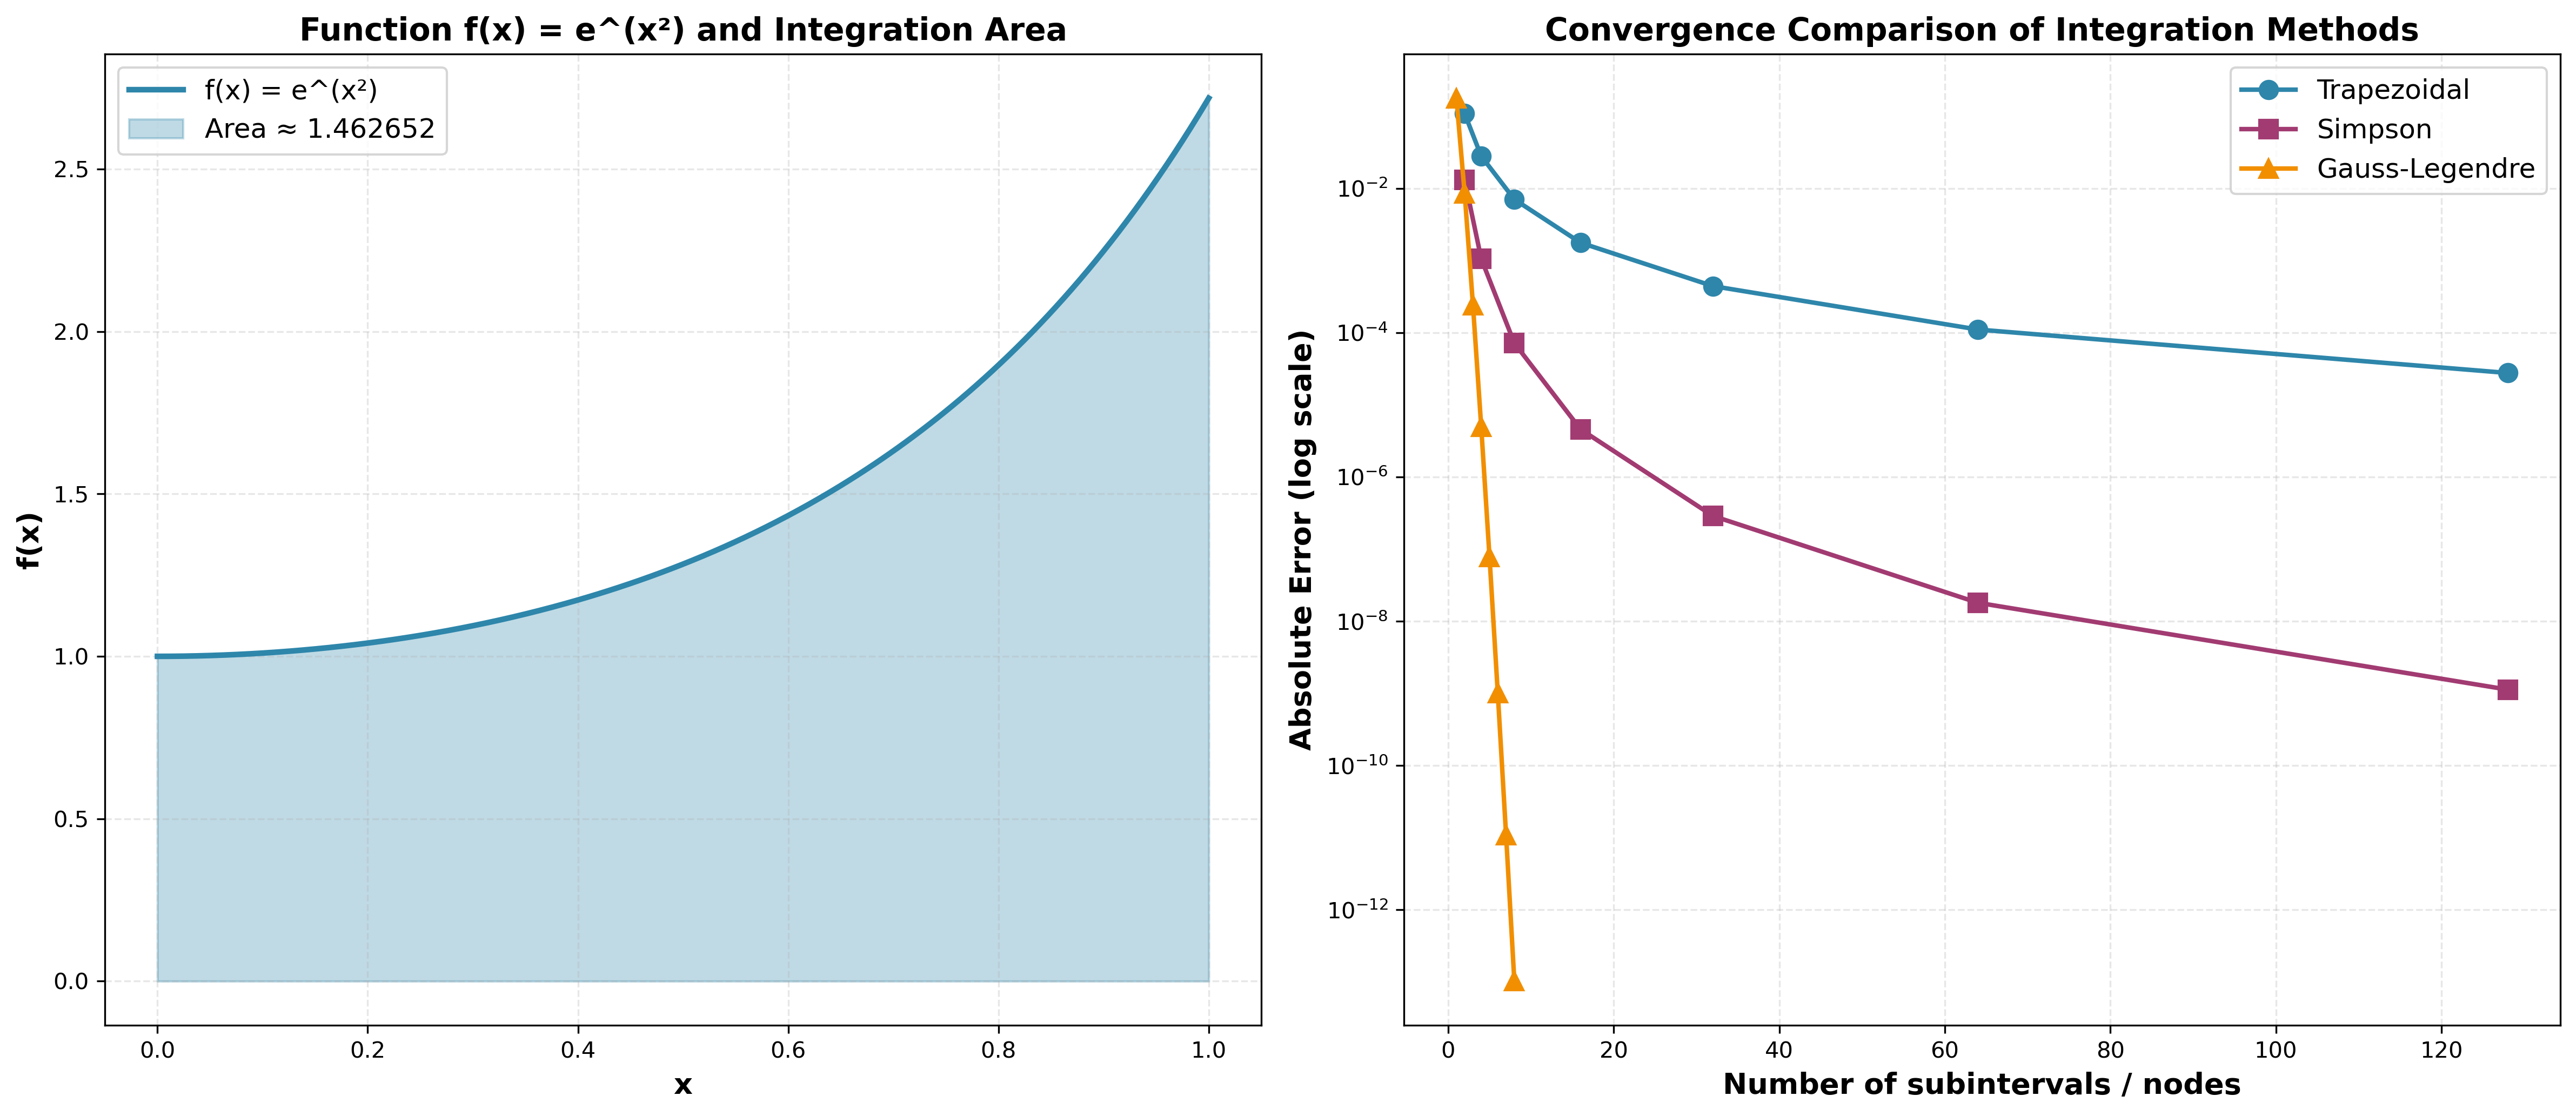
\includegraphics[width=0.88\textwidth]{../outputs/figures/question3_integration.png}
		\caption{Left: area under the function curve. Right: logarithmic comparison of the errors of integration methods}
		\label{fig:integration_plots}
	\end{figure}
	
	\textbf{Conclusion:}
	For a smooth function such as
	$e^{x^2}$,
	the Gauss-Legendre method has the best performance, because it reaches very high accuracy with only a small number of function evaluations. However, if the data are given in tabular form with equal spacing and the analytical function is not available, Simpson's method will be a very suitable and accurate option.
	
\end{document}
